% This is LLNCS.DEM the demonstration file of
% the LaTeX macro package from Springer-Verlag
% for Lecture Notes in Computer Science,
% version 2.3 for LaTeX2e
%
\documentclass[11pt]{llncs}
%
\pagestyle{plain}
\usepackage{makeidx,graphicx,amsmath,verbatim}  % allows for indexgeneration
\usepackage[vlined, ruled]{algorithm2e}


%
\setlength{\topmargin}{-0.3in}
\setlength{\textheight}{8.75in}
\setlength{\oddsidemargin}{0.25in} 
\setlength{\evensidemargin}{0.25in} 
\setlength{\textwidth}{6.00in}

\begin{document}

%
%
\mainmatter              % start of the contributions
%
\title{Hapler Version 1.01}
%
%\titlerunning{Hapler Version 1.01}  % abbreviated title (for running head)
%                                     also used for the TOC unless
%                                     \toctitle is used
%
\author{Shawn T. O'Neil \and Scott J. Emrich}
%
\authorrunning{Shawn T. O'Neil et al.}   % abbreviated author list (for running head)
%
%%%% list of authors for the TOC (use if author list has to be modified)
\tocauthor{Shawn T. O'Neil, Scott J. Emrich}
%
\institute{University of Notre Dame, Notre Dame, IN 46556, USA\\
	\email{\{soneil,semrich\}@nd.edu} 
	}




\maketitle              % typeset the title of the contribution


\setcounter{tocdepth}{3}
\tableofcontents

\newpage

%\begin{abstract}

%\end{abstract}
%

\section{Overview} 
\label{overview}

Suppose you are given a multiple alignment of sequencing reads (such as those that contribute to a consensus contig in an assembly, see Section 
\ref{inputAndOptions}) that represent and unknown number of haplotypes. For example, perhaps you have pooled material for a number of (non-clonal) 
individuals and you sequenced from the ND5 gene of each and aligned them to a reference. Hapler is a tool that attempts to reconstruct these 
haplotypes individually. If there is enough information (high enough coverage, long enough reads, low enough error rates, high enough differentiating 
diversity in the dataset), there is a good chance this can be done. If not, Hapler takes care to only reconstruct shorter haplotype regions it is 
``sure'' of.

For a quick introduction into the basic use of Hapler see Section \ref{exampleUsage}. For considerations on maximizing quality, see section 
\ref{maximizingQuality}.






\newpage

\section{Requirements and Installation}
\label{requirementsAndInstallation}

Hapler is written in Java (as a single .jar file), and has been tested with Java 1.6.0\_22 (on OSX 10.6.6). It is released under the LGPL. To install
and use Hapler, one simply needs to acquire the .jar file and run \texttt{java -jar Hapler.jar} on the command line.





\newpage

\section{Example Usage} 
\label{exampleUsage}

The default options are such that Hapler reads a TIGR formatted multiple alignment on standard input and reconstructs 
haplotypes with 10 coloring repetitions, assuming that all variants define SNP locations:


\begin{verbatim}
 cat pzelicaon_p450_cp6b6_diverse.tigr | java -jar Hapler.jar
\end{verbatim}

Looking at the result of the above by piping into \verb=less -S=, we can see that Hapler returns a lot of information in column/row format, with 
informative comments (lines starting with \verb=#= for easy filtering) describing each column. See Section \ref{output} for more detail about what is 
returned. In this case, because the data was generated by 454, we may wish to use the built-in 454 SNP caller (though for best results SNPs should be
called with external software and inported with \verb=--snp-caller=).

\begin{verbatim}
 cat pzelicaon_p450_cp6b6_diverse.tigr | java -jar Hapler.jar --snp-caller 454
\end{verbatim}

Because Hapler outputs on standard out, we can easily do things such as filter down to high-coverage haplotypes (which our experiments show tend to be
correct):

\begin{verbatim}
 cat pzelicaon_p450_cp6b6_diverse.tigr | java -jar Hapler.jar --snp-caller 454 
                                       | grep -v '^#' 
                                       | awk '{if($15 > 2) print $0}'
\end{verbatim}


Because Hapler can read on standard input, one can easily reconstruct haplotype regions for contigs in an Amos Bank. 
For example, if the file \texttt{eidlist.txt} contains a number of contig identifiers
associated with the Amos Bank \texttt{bank}, one can simply run:

\begin{verbatim}
bank2contig -E eidlist.txt bank | java -jar Hapler.jar --snp-caller 454
\end{verbatim}

Or, using command line sub-shells, two specified contigs:

\begin{verbatim}
bank2contig -E <(echo 7180000019110\\n7180000019111) bank 
                                       | java -jar Hapler.jar --snp-caller 454
\end{verbatim}



\newpage

\section{Input and Options}
\label{inputAndOptions}

Hapler reads multiple alignments in TIGR format (produced by the Amos tools \verb=bank2contig= utility) or SAM format. For examples of these two 
formats, see Appendix \ref{exampleTigrInputFormat} and \ref{exampleSamInputFormat}. If you find bugs in inputting these formats, please let us know. 
Note that Hapler does \emph{not} do the assembly or alignment step for you: you need to produce a TIGR or SAM formatted multiple alignment file 
(either via de-novo assembly or mapping to a reference). More input types may be added in the future.

Although TIGR format does not describe mate-pair information (that we are aware of), SAM format may. Because gaps (e.g. mate-pair information) are 
not compatible with the minimum coloring process (in polynomial time), Hapler will exit with an error should you attempt to use a SAM file with such 
data. This is mostly meant as a reminder: to use such data, use the \verb=--allow-gaps split= option, and sequences containing gaps will be split 
into component contiguous reads. In the case of mate-pairs, this means that mate information is ignored. (Future versions may allow the use of
gaps anyway, though this is expected in most cases to result in very incorrect haplotypes.)

Hapler assumes that \verb=~= characters in either SAM or TIGR sequences are gaps. Otherwise, Hapler is alphabet agnostic: any other non-whitespace
non\verb=~= character can be used in the multiple alignments (for example, one could ``haplotype'' protein sequences). 

Hapler takes the following options:

\subsection{\texttt{--alignment-type <\emph{tigr} or sam>}}

Values can be either \verb=tigr= or \verb=sam=, depending on input type. The default is \verb=tigr=, note that input type is \emph{not}
autodetected.

\subsection{\texttt{--allow-gaps <\emph{false} or split>}}

Values can be either \verb=false= (the default), or \verb=split=. Using a value of \verb=false=, Hapler will exit with an error
if any sequence contains a gap character \verb=~= or the SAM format describes mate-pair information. Using \verb=split= causes gapped data
to be split into component contiguous sequences (and mate-pair information to be ignored). 

\subsection{\texttt{--help}}

Shows a brief description of Hapler and options.

\subsection{\texttt{--input <filename or \emph{-}>}}

The name of the multiple alignment file (SAM or TIGR) to use. If `-' is used (which is the default), Hapler reads on standard input.

\subsection{\texttt{--maximize-one-read-haps <\emph{true} or false>}}

As mentioned in Section \ref{howItWorks}, Hapler samples from minimum colorings of each connected component of the conflict graph.
By default, Hapler searches for minimum colorings which also maximize the number of reads that get colors to themselves: we argue that
since some reads are likely to contain sequencing errors, we have a better chance of isolating them by searching for haplotypes that can 
consist of a single read within the parsimony framework of minimum coloring.

This can be turned off by setting this value to false.

\subsection{\texttt{--random-repetitions <integer>}}

As mentioned in Section \ref{howItWorks}, Hapler samples from minimum colorings of each connected component of the conflict graph.
By repeating these samples and only putting reads together into the same haplotype if they \emph{always} appear together in all
sampled colorings, we can be more sure of the quality of the inference. By increasing the number of samples, we can increase the robustness,
usually at the cost of haplotype length.

Runtime scales roughly linearly with this parameter. Our experiments on gene-size contigs indicate that quality drastically improves for increasing
values from 1-5, improves slowly but noticably from 5-10, and improves very slowly thereafter. Thus, the default is 10, though values of up to 100 
can still be useful.


\subsection{\texttt{--show-alignments}}

Mostly for debugging, this option reports the sections of the multiple alignment contributing to each haplotype reconstruction. Currently
not very user-friendly.

\subsection{\texttt{--snp-caller <\textit{simple}, simplestrict, or 454>}}

For best results, one should use the \emph{--snp-list} option, which overrides this one. Nevertheless, Hapler provides several simple SNP 
calling methods, outlined below:

\begin{itemize}
	\item \texttt{simple}: Any variant locus regardless of allele frequency is treated as a SNP locus.
	\item \texttt{simplestrict}: Any variant locus where a minority allele is present at least twice or is covered by less than 10 reads is treated as a SNP.
	\item \texttt{454}: A variant locus is a SNP if 1) the majority allele is not a `$-$'
	and 2) either a) the number of non-`$-$' alleles is at least two, or
	b) there is any non-`$-$' allele that is not part of a homopolymer run
	of length $\geq 3$.
\end{itemize}

Because the results are fairly dependent on SNP calling and/or error correction accuracy (both in terms of false positives and false negatives), it would
be wise to see section \ref{maximizingQuality}.

\subsection{\texttt{--snp-list <filename>}}

Rather than use the simple built in SNP callers that Hapler provides, the user can provide a list of (0-indexed) loci that describes positions to
use as SNP loci for each multiple alignment. 

This is useful when using external SNP callers, such as QualitySNP or PyroBayes.

For an example of the format taken, see Appendix \ref{exampleSnpInputFormat}.


\newpage

\section{Output}
\label{output}

Hapler outputs information in rows and human readable columns (try using \texttt{less -S} to view the output), with each row corresponding to a 
reconstructed haplotype region. For each multiple alignment, hapler outputs a ``non-variant'' haplotype, consisting of all reads which don't
conflict with any other and representing the non-variant segments of the multiple alignment. After this, variant regions are haplotyped individually
(as haplotype blocks), and a line is shown for each. 

For each multiple alignment, Hapler also outputs a ``SNP Information'' line which begins with a \emph{single} \verb=#= character. This is useful
for viewing SNP locations in the reconstruction column, which are shown in multiple alignment.

\begin{figure}[!h]
\centering
   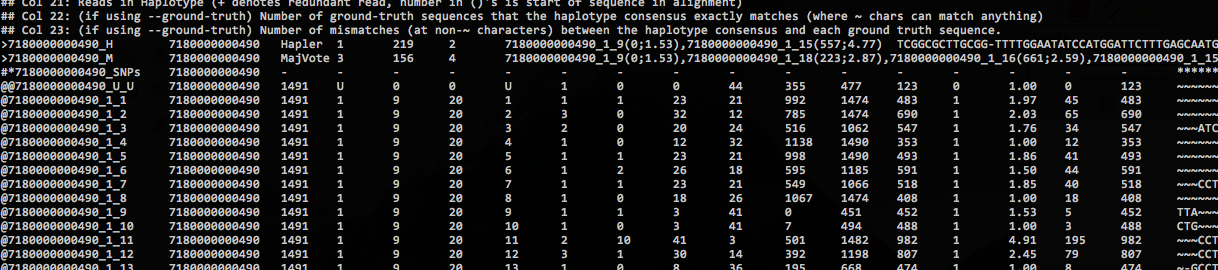
\includegraphics[width=\textwidth]{graphics/hapler_output}
   \caption{A bit of output produced by Hapler.}
   \label{haplerOutput}
\end{figure}


\subsection{Column 1 - Unique Haplotype Identifier}

This column gives a unique identifier for each reconstructed haplotype region, which is merely a concatenation of the next three columns.

\subsection{Column 2 - Multiple Alignment Name}

Each haplotype or haplotype block is associated with its input multiple alignment name (from the TIGR or SAM file) through this column.

\subsection{Column 3 - Haplotype Block Number}

Non-variant regions seperate connected components in the conflict graph (see Section \ref{howItWorks}). When there are such non-variant regions 
(multiple connected components), we have no information to attach haplotypes from one variant region to another. Thus, each haplotype reconstruction
is associated with the variant region, or ``Haplotype Block,'' it belongs to through this column. These are numbered, for each multiple alignment, 
beginning at 1.

This value is `U' for the ``non-variant'' Haplotype, which isn't technically associated with any block.

\subsection{Column 4 - Minimum Number of Haploytypes Supported By Block}

Parsimony suggests that we should minimally color the conflict graph (see Section \ref{howItWorks}), equivalent to reconstructing a 
minimum number of haplotype regions supported by the data. However, because we repeat and sample the coloring process, we usually
end up with a larger number of haplotype reconstructions. This number, which is the same for all haplotypes in a single block (it's really
associated with the haplotype block, rather than haplotypes), gives the minimum number that would be constructed by pure parsimony (a single 
sampling).

\subsection{Column 5 - Haplotype Number}

Within each haplotype block, each haplotype is given a number, counting upward from 1. The ``non-variant'' haplotype is given the special
designator `U'.

\subsection{Column 6 - Number of Non-Redundant Sequences}

In order to minimally color the conflict graph, Hapler must ``mask'' redundant reads (those whose covered SNP loci are a subset of some other 
non-conflicting read). This masking is done by the reads themselves: if read A makes read B redundant, and read B makes read C redundant,
then A must also make C reduntant: so A ``masks'' B and C and these are removed from the haplotyping process.

This column then gives the number of non-redundant (non-masked) reads associated with each haplope reconstruction.

\subsection{Column 7 - Number of Redundant Sequences}

As a compliment to Column 6, we also give the number of redundant reads associated with reads contributing to each haplotype reconstruction.

\subsection{Column 8 - Number of Defined SNPs Covered}

A read is said to \emph{cover} a SNP locus if it has a known allele (non-`~' character) there. The number of SNPs defined by a haplotype region
is the union of those covered by all reads within it.

\subsection{Column 9 - Number of Covered, Inconsistent SNPs}

Currently, this value will always be 0. Future versions of Hapler may allow for the consideration of gapped reads (e.g. mate pair information), but 
in this case some reconstructed haplotypes may contain conflicting alleles at SNP loci (since this breaks the minimum coloring foundations). This 
column will count these inconsistencies.


\subsection{Column 10 - Number of Defined SNPs Not Covered}

The total number of defined snps for the multiple alignment minus column 8. 


\subsection{Column 11 - Start Position of Haplotype}

This is the 0-indexed position of the first non-`~' character in the haplotype consensus (i.e., the first position of the first read in the haplotype).
If there are no reads in the haplotype (this can only happen with the non-variant `U' haplotype), this will be -1.

\subsection{Column 12 - End Position of Haplotype}

This is the 0-indexed position of the last non-`~' character in the haplotype consensus (i.e., the last position of the last read in the haplotype).
If there are no reads in the haplotype (this can only happen with the non-variant `U' haplotype), this will be -1.

\subsection{Column 13 - Length of Haplotype}

End Position - Start Position + 1, unless no sequences are in the haplotype (this can only happen with the non-variant `U' haplotype)), in which case 0.

\subsection{Column 14 - Number of Pieces Haplotype Is In}

Because of the minimum coloring formulation, it is possible for a haplotype to consist, for example, of only two reads that are far apart in the multiple
alignment. If these two always share a coloring, we can be confident of their association, even though there is no ``positive'' information (shared SNP
alleles) linking them (see Section \ref{howItWorks}).

Pieces represent association not only via coloring but also via positive shared SNP allele information: pieces are defined as connected components in
an overlap-at-SNP loci graph within haplotypes. Thus, for any two reads which are part of the same piece, there is a path over overlapping and agreeing
SNP allele reads between them.

Multiple pieces indicate a lack of such positive information linking reads together within a reconstructed haplotype, even though the
repeated coloring may suggest they belong to the same haplotype.  Usually, however, the repetition
of colorings forces haplotypes down to a single piece.

\subsection{Column 15 - Average Sequence Coverage of Haplotype}

The is similar to the ``average gapped coverage'' used in assembly. We take the total number of bases represented in reads belonging to the haplotype
(\emph{including} redundant/masked reads), and divide it by the length of the haplotype (see above). Note that if a haplotype doesn't determine some
inside section (which can only happen if it is in multiple pieces), then this value can be below 1.0.

\subsection{Column 16 - Haplotype Consensus at SNP Positions}

This column shows the reconstructed haplotype regions, with all non-SNP loci removed. It provides a good summary of the haplotypes created and their
length/coverage relative to the variant loci. These are shown aligned for all variant loci: where a haplotype doesn't determine an allele
a `~' character is used.

Consensus bases for each SNP locus are called as the majority vote of reads within each haplotype (which will always agree unless there are Inconsistent
SNPs, see above).

\subsection{Column 17 - Full Haplotype Consensus}

The column shows the reconstructed haplotypes, including non-variant loci, all aligned against each other. Where a haplotype isn't determined,
`~' characters are used.  

Consensus bases for each SNP locus are called as the majority vote of reads within each haplotype (which will always agree unless there are Inconsistent
SNPs, see above). Consensus bases for all other loci are called as the majority vote of all reads in the multiple alignment: this helps filter out
sequencing errors which have not been called as SNP loci, since per-haplotype coverage is often low.

\subsection{Column 18 - Reads In Haplotype}

For each reconstructed haplotype, Hapler also reports the reads contributing to it. Read IDs that are prefixed with a `+' are redundant
and are masked by the preceeding non-`+' read. For each read, the start position in the multiple alignment (0-indexed) is also given in 
parentheses. 


\newpage
\section{Maximizing Quality}
\label{maximizingQuality}

In general, for hapltyping applications, poor data can still result in 1) possible sequencing error being included in haplotype
reconstructions, 2) chimeric haplotype reconstructions, 
Hapler uses a repeated, weighted bipartite matching method to try and maximize the robustness of the returned haplotype regions (see Section 
\ref{howItWorks} and \cite{ONEIL2011}): although sequencing errors can still get through (these are often represented as single read 
haplotypes, and sometimes as longer haplotypes with low coverage) and chimeras can still exist, this usually results in shorter haplotypes being returned,
representing uncertainty in the data.

Thus, for best results, one should still consider the quality of data fed to Hapler.

\subsection{Read Length and Coverage}

If no read spans a non-variant region, Hapler will not attempt to build haplotypes across that region. Thus, it is necessary to 1) use long enough
read lengths that non-variant regions can be spanned by reads, and 2) have high enough coverage that this does actually happen. An estimation of 
read length and coverage necessary to do this can be found in \cite{ERIKSSON2008}. Ideally, one would want high enough coverage that all regions
of all haplotypes are covered to some degree. One of the benefits of Hapler is that if such data isn't available, it will work with what you do have
and not return answers that aren't well-supported.

\subsection{SNP Calling and Error Correction}

Our experiments with Hapler indicate that sequence quality and locating true SNPs is of quite high concern if one wants accurate haplotype 
reconstructions. Hapler determines errors from non-errors through the calling of SNP-loci: variations at SNP-called loci define the conflict 
information, while other variations (which are presumably errors) are ignored, though left in the original data.

Notably, both false-positive and false-negative SNP calls can adversely affect haplotyping performance. A false-negative SNP (a true SNP that is 
mistaken for a sequencing error) means that some genetic variation will be ignored. This can result in a haplotype missing from the output, or a 
possible chimera because that diversity may have allowed for differentiation that is consequently ignored.

False-positive SNPs (calling errors as SNPs) are troublesome as well-these can be viewed as erroneous, rare haplotypes supported by only a single 
read. This is variation that Hapler will attempt to isolate through the ``maximizing single-read haplotypes'' mechanism. Even so, it is possible for 
these erroneous reads to ``stick to'' other, correct reads that they share correct alleles with, resulting in longer (though usually low average 
coverage) haplotypes. Although a coverage-cutoff often identifies these (see \cite{ONEIL2011}), this is a waste of the correct reads that are 
stuck to the erroneous reads, reducing haplotype information amongst correct reads.

Finally, we note that calling SNPs is generall much harder when coverage is low, as near the ends of assembled contigs. Thus, one may want to 
``trim'' multiple alignments so that coverage is high throughout. Further, even if errors are not called as SNPs, if they sit in regions with 
locally low coverage (2x or smaller), Hapler may use the errors as the base call of the overall multiple alignment, causing the error to be
present in all haplotypes spanning that region.

\subsection{Sampling Number}

As described in Section \ref{howItWorks}, Hapler samples in a pseudo-random fashion from minimal coloring solutions, keeping only common
haplotype information: an increase in repetitions with the \texttt{--random-repetitions} parameter results in higher confidence of the
reconstructions. As shown in \cite{ONEIL2011}, for a single coloring many long but chimeric haplotypes are created. Increasing the
parameter to 5 rapidly decreased the number of such chimeras (at a cost of haplotype reconstruction length), and increasing to 10 further
improved the results but at a slower rate, becoming nearly asymptotic. Thus, the default for this parameter is 10, even though other tests
in \cite{ONEIL2011} were run with 100 repetitions. These tests were run with simulated 5x per haplotype coverage of an approximately 2800bp
gene: larger datasets may require more repetitions.

Currently, we recommend increasing the repetition number until the number of reconstructed haplotypes stabilizes. We hope to include this 
functionality automatically in future releases.




 
\newpage

\section{How it works}
\label{howItWorks}

The following is a quick, intuitive overview. More details can be found in \cite{ONEIL2011}. We are grateful for the work done by Eriksson et al. 
(\cite{ERIKSSON2008}): Hapler expands on the initial graph-theoretical formulation proposed there for increased robustness on low-coverage, low-diversity
data.

Haplotyping is done primarily by creating a graph with each read corresponding to a node such that two nodes are connected by an edge if they conflict. If 
we minimally color this graph, each color consists of nodes that don't conflict and may represent data sourced from the same haplotype. Note that by this 
formulation reads which don't overlap can be given the same color, thus haplotype reconstructions can return ``gaps'' in the middle. For example the
``red'' reads in Figure \ref{exampleConflictGraph} leave an undefined section between the first and second read. This is infrequent in normal usage: 
\emph{usually} this indicates uncertainty caused by lack of coverage or genetic diversity which Hapler is designed to avoid (see below).

%% Figure of multiple coloring
\begin{figure}[!h]
\centering
   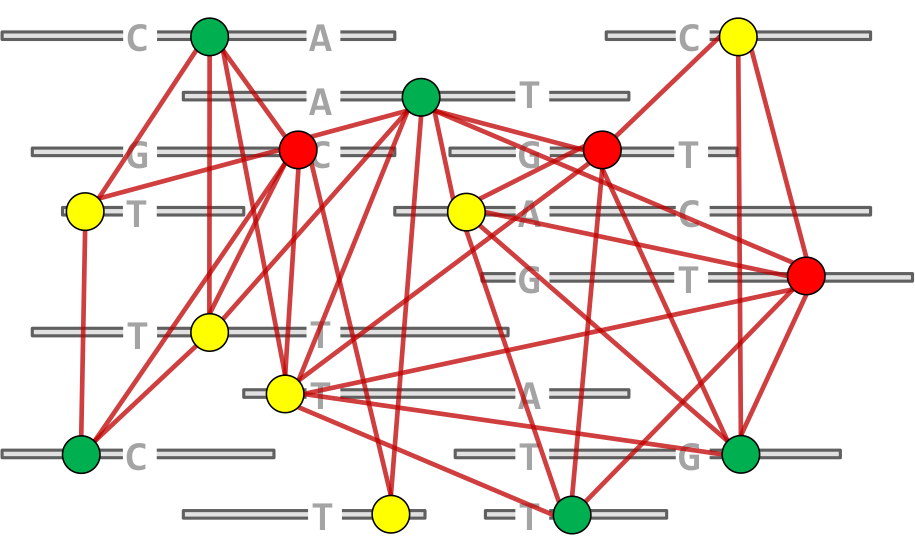
\includegraphics[width=0.4\textwidth]{graphics/mincolor}
   \caption{Given a multiple alignment of reads (here showing only positions defined as SNPs), we want to create a conflict graph and minimally color it.}
   \label{exampleConflictGraph}
\end{figure}



Minimum coloring is generally NP-hard. However, if ``gaps'' (unknown sequence) are not allowed in the reads (where a gap in a read precludes conflicts at the 
unknown alleles), then this problem is polynomial time. Note that mate-pairs could be considered as single a single sequence with a large gap in the 
middle: ideally, we'd like to use a single graph node to represent both ends of the mated read. Unfortunately, to ensure polynomial time and correct 
answers, we have to use two nodes, thus each end may end up in different haplotypes. 

\begin{figure}[!h]
\centering
   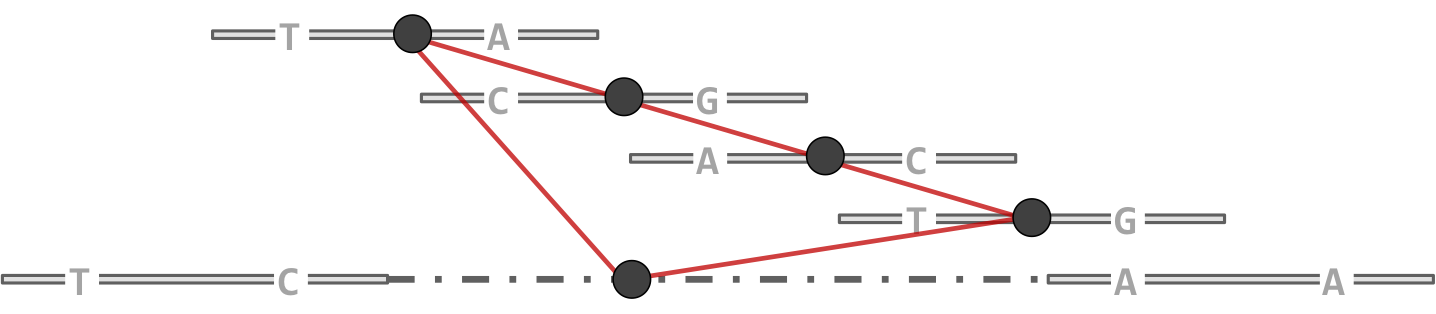
\includegraphics[width=0.6\textwidth]{graphics/mate-pair}\\
   NP-Hard\\
   \vspace{1em}
   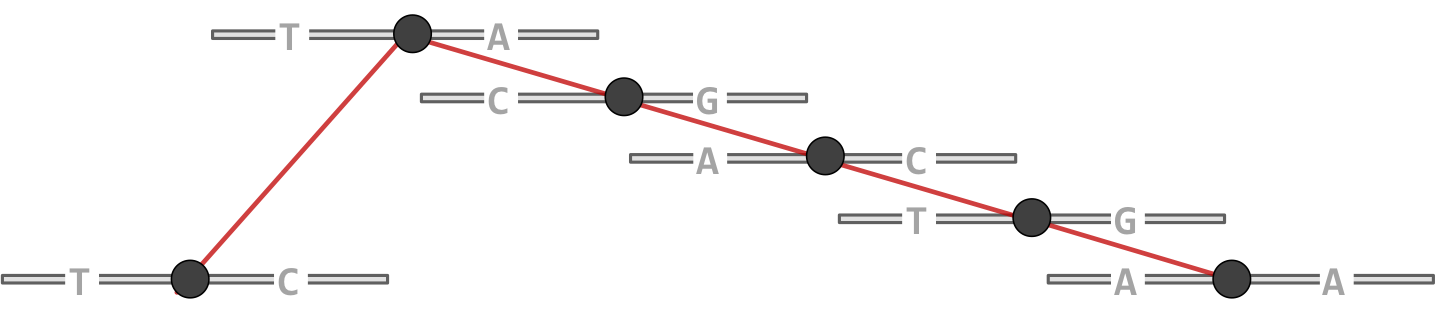
\includegraphics[width=0.6\textwidth]{graphics/mate-pair_broken}\\
   Polynomial Time
   \caption{The minimum coloring problem is polynomial time in this case if we ensure that reads are contiguous, without ``gaps.'' This, however, 
   means that mate-pair information cannot be fully used: we must associate mated reads with different graph nodes, such that they can possibly
   be associated with different haplotypes.}
   \label{matePairs}
\end{figure}


%% Figure of mate-pair NP-hard version

%% Figure of mate-pair easy version

Hapler executes a number of steps, which can be summarized as follows:
\begin{enumerate}
	
	\item SNP-call. We may wish to only consider some variations as relevent for haplotyping, to ignore sequencing errors, for example. Hapler can 
	take a list of positions to use as SNPs, or can find it's own using a variety of methods (see Section \ref{inputAndOptions}).
	
	\item Identify reads that don't conflict with anything. These reads are common to all haplotypes, are are collected together into a ``non-variant''
	haplotype that may have several gaps (where variation occurs).
	
	\item Identify haploytpe blocks. If reads are too short to span invariant regions, then there is no way to associate a haplotype segment from
	one variant region to another. (More formally, we only perform haplotyping on connected components of the conflict graph).

\begin{figure}[!h]
\centering
   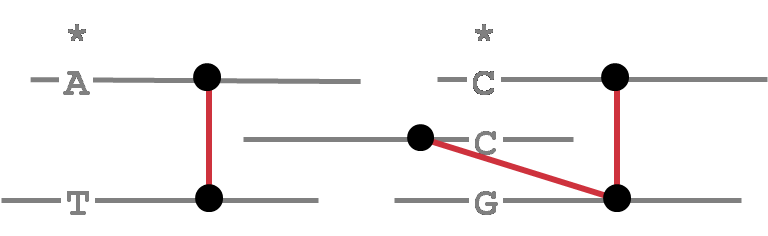
\includegraphics[width=0.4\textwidth]{graphics/haplotype_blocks}
   \caption{If there is more than one connected component in the conflict graph, no information exists to associate haplotypes from
   one connected component to another. Thus, Hapler only reconstructs haplotype regions for reads that are part of the same connected 
   component, which form contigious ``haplotype blocks.'' Reads which occur between these and conflict with nothing are part of invariant
   regions; these are associated with a special ``non-variant'' haplotype for each multiple alignment (see Section \ref{output}).}
   \label{bicolor}
\end{figure}

	
	\item Minimally color the haplotype block conflict graphs. Hapler by default finds minimim colorings that also maximize the number of nodes 
	(reads) given colors all to themselves (reads that define a haplotype all by themselves). Since sequences containing errors could be veiwed as 
	``haplotypes unto themselves,'' this is an effort to isolate sequencing error. (See Figure \ref{alternatecoloring}).	
	
	\item Repeated coloring. Because multiple such colorings (haplotypings) may be possible, Hapler repeats this process a user-specified number of 
	times, and only puts two reads into the same haplotype if they always are put together by the colorings. Increasing this parameter increases the
	confidence of haplotypes, avoiding chimeric reconstructions.
	
\begin{figure}[!h]
\centering
   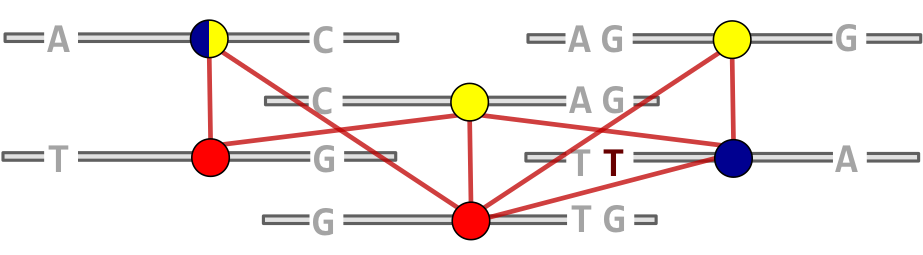
\includegraphics[width=0.4\textwidth]{graphics/two_haps_bicolor}
   \caption{There are many ways to minimally color a conflict graph; Hapler by default finds ways that also maximize the number of reads which 
   are left as colors (haplotypes) unto themselves. In this example, the upper left read may be given two possible colors: Hapler forces the use of
   yellow. This can be turned off by using \texttt{--maximize-one-read-haps false} (see Section \ref{inputAndOptions}). 
   Even so, in general multiple solutions may still be possible: Hapler psuedo-randomly samples from these and only infers haplotypes
   for reads which always appear similarly colored. The number of such samples is controlled with the \texttt{--random-repetitions} option.}
   \label{alternatecoloring}
\end{figure}

	
	\item Haplotype consensus. For each haplotype a consensus is created, which is only defined for regions that are covered by reads assigned to the 
	haplotype. Undefined regions are left as `~'. For SNP-called loci, the majority allele within the haplotype (which will be invariant unless the
	\texttt{--allow-gaps true} option is used with gapped data, see Section \ref{inputAndOptions}) is used for the call. For Non-SNP-called loci, the majority
	vote of the alignment as a whole is used--this usually prevents sequencing error from getting into the haplotype reconstructions, since coverage 
	will be high overall but low for each individual haplotype.

\end{enumerate}



\appendix

\newpage
\section{Example TIGR Input Format}
\label{exampleTigrInputFormat}

The TIGR alignment format describes a multiple alignment of short reads against one or more longer consensus sequences. It is output by the Amos
tool \texttt{bank2contig} when working with an Amos Bank. 
For example, if the file \texttt{eidlist.txt} contains a number of contig identifiers
associated with an Amos Bank \texttt{bank}, one can simply run:

\begin{verbatim}
bank2contig -E eidlist.txt bank | java -jar Hapler.jar
\end{verbatim}

The TIGR format describes each multiple alignment starting with a \verb=##= line describing each consensus, followed by a number of \verb=#=
lines describing the placement of each read. Here is an example:

\begin{figure}[!h]
\centering
   \includegraphics[width=0.6\textwidth]{graphics/Example_tigr}
   \caption{Screenshot of example TIGR formatted input.}
   \label{exampleTIGR}
\end{figure}

Hapler currently only uses the following information from this format:  Contig IDs (for the multiple alignment names, \texttt{7180000000490} in the above),
Read Names (\texttt{FQVI7FG02F5V01} etc.), gapped read sequences, and read placement (numbers in \texttt{()}s: \texttt{239} and \texttt{452} in the above).

\newpage
\section{Example SAM Input Format}
\label{exampleSamInputFormat}

SAM is a relatively recent ASCII-formatted description of assembly/alightments. Each line represents a single read (which may be mated with another
read described in another line). Formal documentation can be found in \cite{LI2009}. The general form for each line is whitespace separated columns 
describing:

\begin{enumerate}
	\item Read Name
	\item Flag
	\item Scaffold Name
	\item Start Position (0 indexed, IIRC)
	\item Map Quality
	\item CIGAR alignment string
	\item Mate Name
	\item Mate Position
	\item Insert Size
	\item Ungapped Sequence
	\item Quality Sequence
\end{enumerate}

SAM format specifies that mated reads will be given the \emph{same} name: this is how Hapler determines the existence of mate-pairs. 
When using the \texttt{--allow-gaps split} option, each read of a mate pair will be given a unique name by appending a number to the name:
\verb=_0=, \verb=_1=. (If there are multiple reads with the same name, this numbering scheme can continue).

\begin{figure}[!h]
\centering
   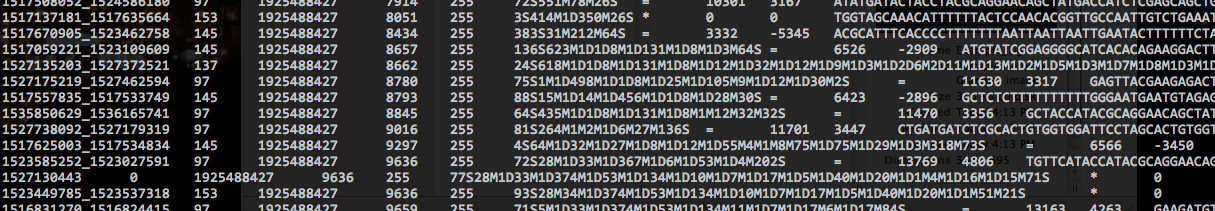
\includegraphics[width=\textwidth]{graphics/Example_sam}
   \caption{Screenshot of example SAM formatted input.}
   \label{exampleSAM}
\end{figure}

Hapler uses the Read Name and Start Position columns when parsing data. For the CIGAR string, the \verb=S= command necessitates a Soft Clip (sequence
at the start or end that should be ignored), which is honored by Hapler. Hard clips (\verb=H=) are assumed to have already been done to reads, so
Hapler ignores these. Values of \verb=N= are replaced with \verb=~= characters, which will cause an error unless \texttt{--allow-gaps split} is set, in 
which case the sequences will be later split into seperate sequences at those positions. Insert characters (\verb=I=) are not allowed: Hapler
assumes that the multiple alignment is ``gapped.'' \verb=D= characters, which indicate deletion alleles w.r.t. the reference, cause Hapler to 
insert \verb=-= characters into the sequence. And of course, match characters (\verb=M=) are used to reconstruct the full gapped sequence from
the ungapped sequence. 

Hapler ignores Quality information in its current form.


\section{Example SNP Input Format}
\label{exampleSnpInputFormat}

Ok, you got me. This feature hasn't been implimented yet. Soon! I promise!


\bibliographystyle{plain}
\bibliography{khap}


\end{document}
